\documentclass[]{article}
\usepackage[a4paper,top=3cm,bottom=3cm,left=3cm,right=3cm]{geometry}

\usepackage{amsmath}
\usepackage{mathtools}
\usepackage{bm}
\usepackage{amsfonts}
\DeclareMathOperator*{\argmin}{argmin}
\DeclareMathOperator*{\argmax}{argmax}
\usepackage{graphicx}
\usepackage{grffile}
\usepackage[colorlinks=true, allcolors=blue]{hyperref}
\usepackage{amsthm}
\usepackage{enumitem}
\usepackage{physics}
\usepackage{tabularx}
\usepackage{float}
\usepackage[font=small]{caption}
\usepackage[export]{adjustbox}

\newcommand{\w}{\mathbf{w}}
\newcommand{\x}{\mathbf{x}}
\newcommand{\bbeta}{\boldsymbol \beta}

\newtheorem{theorem}{Theorem}[section]
\newtheorem{corollary}{Corollary}[theorem]
\newtheorem{lemma}[theorem]{Lemma}
\newtheorem{remark}[theorem]{Remark} 

\graphicspath{{/home/zc21901/Courses/SC and SM 1/group project/higgsboson}}

%opening
\title{Tuning of logistic regression for Higgsboson ML challenge}
\author{Ettore Fincato, Hannah Sansford, Harry Tata}



\begin{document}

\maketitle

\begin{abstract}

We investigate the tuning of a logistic regression for finding evidence of the decay into \textit{fermion} pairs of the Higgs Boson, for the Higgs Boson Machine Learning Challenge \cite{higgs-challenge}. With the aim of finding a logistic classification maximising the AMS objective function \ref{AMS}, we show a tuning based on a two-stage procedure from \cite{kotlowski2014consistent}. This tuning strategy relies on a first stage where we fit the logistic model coefficients, and on a second stage where we tune a classification threshold on the basis of AMS. Being able to show that AMS values based on the two-stage procedure are significantly bigger than the ones based on the standard logistic classification threshold, we can state that the coefficients from the logistic model can still be considered. Logistic regression is a simple model with a straightforward coefficients interpretation, which is convenient for a setting in which the variables have a physical interpretation.

\end{abstract}

\section{Introduction}

\subsection{Background}

The Higgs boson can \textit{decay} through various different processes, producing other particles in the process. In physics, one calls a decay into specific particles a \textit{channel}. Until fairly recently, the Higgs boson had been seen only in boson pair decay channels. It is now of importance to seek evidence on the decay into \textit{fermion} pairs, specifically \textit{tau-leptons} or \textit{b-quarks}, and to measure their characteristics \cite{higgs-challenge}. The ATLAS experiment \cite{ATLAS-experiment} was the first to report evidence of the \textit{H} to tau-tau channel and the goal of this report is to improve on this analysis.


\subsection{Overview}

The Atlas experiment at CERN provided simulated data that was used to optimise the analysis of the Higgs boson. In the Large Hadron Collider (LHC), proton bunches are accelerated in both directions on a circular trajectory. This results in some of the protons colliding as the bunches cross the ATLAS detector (called an \textit{event}), which produces hundreds of millions of proton-proton collisions per second. The particles resulting from each event are detected by sensors and, from this raw data, certain real-valued features are estimated \cite{higgs-challenge}.

Most of the uninteresting events (called the \textit{background}) are discarded using a real-time multi-stage cascade classifier. However, many of the remaining events represent known processes that are also known as \textit{background}. Our aim is to find the region of the feature space in which there is a significant excess of events compared to what known background processes can explain (called \textit{signal}).

Once the region has been fixed, the significance of the excess is determined using a statistical test. If the probability that the excess has been produced by background processes falls below a pre-determined limit, the new particle is deemed to be discovered.




\section{Problem Formulation}

Let $\mathcal{D} = \{(\bm{x}_1, y_1,w_1),...,(\bm{x}_n,y_n,w_n)\}$ the the training set, where $\bm{x}_i \in \mathbb{R}^d$ is a $d$-dimensional feature vector, $y_i \in \{\text{b,s}\}$ is the label, and $w_i \in \mathbb{R}^+$ is a non-negative weight. Let $\mathcal{S} = \{i : y_i = \text{s}\}$ and $\mathcal{B} = \{i : y_i = \text{b}\}$ be the index sets of signal and background events respectively, and let $n_\text{s} = |\mathcal{S}|$ and $n_\text{b} = |\mathcal{B}|$ be the number of simulated signal and background events. 

The simulated dataset also includes importance weights for each event. Since the objective function (\ref{AMS}) depends on the \textit{unnormalised sum} of weights, in order to make the setup invariant to the \textit{numbers} of simulated events $n_s$ and $n_b$, the sum across each set (test/training) and each class (signal/background) is set to be fixed, i.e.,
\begin{equation}
	\sum_{i \in \mathcal{S}} w_i = N_\text{s} \hspace{10pt} \text{and} \hspace{10pt} \sum_{i \in \mathcal{B}} w_i = N_\text{b}.
\end{equation}
These normalisation constants $N_\text{s}$ and $N_\text{b}$ are simply the \textit{expected total number} of signal and background events, respectively, during the time interval of the data taking. The individual weights are then proportional to the conditional densities,
$$ p_\text{s}(\bm{x}_i) = p(\bm{x}_i|y=\text{s}) \hspace{10pt} \text{and} \hspace{10pt} p_\text{b}(\bm{x}_i) = p(\bm{x}_i|y=\text{b}), $$
divided by the instrumental densities $q_\text{s}(\bm{x}_i)$ and $q_\text{b}(\bm{x}_i)$, i.e.,
\begin{equation}
	w_i \propto \begin{cases}
	p_\text{s}(\bm{x}_i)/ q_\text{s}(\bm{x}_i), & \text{if} \hspace{10pt} y_i= \text{s}. \\
	p_\text{b}(\bm{x}_i) / q_\text{b}(\bm{x}_i), & \text{if} \hspace{10pt} y_i= \text{b}.
	\end{cases}
\end{equation}


Now, let $g: \mathbb{R}^d \to \{\text{b,s}\}$ be a classifier. Let the \textit{selection region} $\mathcal{G} = \{\bm{x}: g(\bm{x}) = \text{s}\}$ be the set of points classified as signal, and let $\hat{\mathcal{G}}$ denote the \textit{index set} of points that $g$ classifies as signal, i.e.,
$$ \hat{\mathcal{G}} = \{i:f(\bm{x}_i) \in \mathcal{G}\} = \{i : g(\bm{x}_i) = \text{s}\}. $$
Then we have that
\begin{equation}
\label{s weights}
	s = \sum_{i \in \mathcal{S} \cap \hat{\mathcal{G}}} w_i
\end{equation}
is an unbiased estimator of the expected number of signal events selected by $g$, and similarly,
\begin{equation}
\label{b weights}
b = \sum_{i \in \mathcal{B} \cap \hat{\mathcal{G}}} w_i
\end{equation}
is an unbiased estimator of the expected number of background events selected by $g$. Alternatively, $s$ and $b$ are the \textit{unnormalised} true and false positive rates, respectively.

High-energy physicists suggest the use of the \textit{approximate median significance} (AMS) objective function defined by
\begin{equation}
\label{AMS}
	\text{AMS} = \sqrt{2 \left[ (s + b + b_\text{reg}) \ln \left( 1 + \frac{s}{b + b_\text{reg}} \right) - s \right]}
\end{equation}
to optimise the selection region for discovery significance, where $b_\text{reg}$ is a regularisation term suggested to be set to $b_\text{reg}=10$. Hence, our aim is simply to train a classifier $g$ based on the training data $\mathcal{D}$ with the goal of maximising the AMS on some unseen test data.

\section{Maximising the AMS}

Having decided a statistical model for classification, its parameters will be tuned by maximising the AMS. This can be done in two ways.

\begin{itemize}
\item \textbf{Direct maximisation}: One can consider the AMS as an error/objective measure in a cross validation procedure. So the model will be tuned by a cross validation (cv) procedure by looking at the coefficients which directly maximise the AMS.

\item \textbf{Two-stage maximisation}: Given a real-valued function $f$ (e.g. a linear $f(\bm{w},\bm{x})=\bm{w}'\bm{x}$), one can always get a classification model by setting a threshold $\theta \in A\subset \mathbb{R}$ and a classifier
\begin{equation}
\label{classifier from f}
h(\theta):=\operatorname{sgn}(f-\theta)\in \{-1,1\}
\end{equation}
One can therefore train and tune $f$ ``independently" of the AMS, and then find the threshold $\theta$ for which the classifier $h(\theta)$ maximises the AMS. For example, one could train $f$ in a logistic regression (i.e. train $f$ s.t. it minimises a logistic loss), and then, on a second stage, choose the classification threshold based on AMS. This approach is presented in \cite{kotlowski2014consistent}
\end{itemize}
We will see that the two-stage maximisation is much more performant (in terms of AMS) than the direct one.

\subsection{Two-stage maximisation}

While the direct maximisation with cv can be seen as a usual tuning procedure by cross validation, the two-stage maximisation should be justified. This section is dedicated to the explanation of the two stage procedure for a  classifier $h:\mathcal{X}\to \{-1,1\}$, as defined in (\ref{classifier from f}) , where $\mathcal{X}$ denotes the features space, and \textbf{$f$ is trained by minimising a logistic loss}.\\

By incorporating the weights to the probabilities, without loss of generality one may write  $s$ and $b$ from (\ref{s weights}) and (\ref{b weights}) as

$$s=s(h):=\mathbb{P}(h(\bm{X})=1,Y=1) \ \text{,} \ \ \ b=b(h):=\mathbb{P}(h(\bm{X})=-1,Y=1)$$
where $\bm{X}$ denotes a random imput vector and $Y$ a random binary response. The paper justifies the two stage procedure explained above for logistic loss transformation of $f$, as follows. Given a classifier $h$ obtained from $f$ as in (\ref{classifier from f}), one can define the``AMS regret" as
\begin{equation}
\label{regret}
R_{AMS}(h):= \text{AMS}^2(h^*)-\text{AMS}^2(h)
\end{equation}
where $$h^*:=\underset{h}{\text{argmax}} \ \text{AMS}^2(h).$$
Similarly, the``logistic regret" of $f$ is defined as
\begin{equation}
\label{logistic regret}
R_{log}(f):= L(f)-L(f^*)
\end{equation}
for the expected logistic loss transformation of $f$ 
\begin{equation}
\label{eq: logloss}
L(f):=\mathbb{E}\Big[\log(1+e^{-Yf(\bm{X})})\Big]
\end{equation}
and $$f^*:=\underset{f}{\text{argmin}} \ L(f)$$
The formal justification of the idea of 
\begin{itemize}
\item training a logistic loss transformation of $f$, and
\item finding the threshold $\theta$ in \ref{classifier from f} by maximising the AMS on a second stage
\end{itemize}
comes from the following theorem.

\begin{theorem}
\label{thm: two stage maximisation}
Given a real-valued function $f$ and the related classifier $h(\theta):=\operatorname{sgn}(f-\theta)$,  let $\hat{\theta}:=\underset{\theta}{\operatorname{argmax}} \ \operatorname{AMS}(h)$. Then,
\begin{equation}
\label{regret inequality}
R_{AMS}(h(\hat{\theta}))\leq \frac{s(h^*)}{b(h^*)}\sqrt{\frac{1}{2}R_{log}(f)}
\end{equation}

\end{theorem}
\begin{proof}
 See \cite{kotlowski2014consistent}-Theorem 2.
\end{proof}

That is, the AMS regret of classifier $h(\theta)$ is upper bounded by the logistic regret of the underlying $f$. It is possible to prove that it is sufficient to optimize $\theta$ on the empirical counterpart of AMS calculated on a separate validation sample. 


\begin{remark}
Training $f$ by minimising a logistic loss is particularly suited for a classification task. For example, it allows us to train (on the first stage) models such as a logistic regression. 
\end{remark}
\begin{remark}
As far as logistic regression is concerned, recall that after model's coefficients $\bm{w}$ have been estimated, classification for a new observation $y_0$ can be done by setting  $\hat{\bm{w}}'\bm{x}_0>\theta$ for some suitable $\theta \in \mathbb{R}$. In a "proper" logistic regression, $\theta$ is directly set to $0$. Here we choose it during a second stage via maximising AMS.
\end{remark}

Our aim is to tune a logistic regression. The theoretical set-up of logistic regression can be found below.

\subsection{Logistic regression}


Suppose $y\in \{-1,1\}$. Note that
\begin{align}
p(y=1|\x)&=\frac{p(\x|y=1)p(y=1)}{p(\x|y=1)p(y=1)+p(\x|y=-1)p(y=-1))} = \frac{1}{1+\frac{p(\x|y=-1)p(y=-1)}{p(\x|y=1)p(y=1)}}
\end{align}
Logistic regression is a discriminative learning model which aims at minimising an expected loss by predicting 
$$\hat{y}=\operatorname{argmin}_{y_0}\mathbb{E}_{p(y|\x)}(L(y,y_0)|\x)$$
and by \textit{inferring $p(y|\x)$ directly}. \\


Specifically, it models the log density ratio as 

$$\log\Big(\frac{p(\x|y=-1)p(y=-1)}{p(\x|y=1)p(y=1)}\Big)\overset{model}{=}f(\x,\bbeta):=\langle \bbeta,\x \rangle+\beta_0$$ 

i.e. models the "log-odds"  by a linear model (the term on the left of the proportionality symbol is added for intuition). In this way we can write 
\begin{align}
p(y|\x;\bbeta)=\sigma(f(\x,\bbeta)y)
\end{align}
for a so-called "activation/logistic function" $\sigma(t):=\frac{1}{1+\exp(-t)}$.  \\
ML estimates of $\bbeta$ are computed from the log-likelihood as $$\bbeta_{ML}=\operatorname{argmax}_{\bbeta}\sum_{i\in D}\log\sigma(f(\x_i,\bbeta)y_i)$$

\begin{remark}
Notice that 
\begin{align*}
\text{argmax}\sum_{i\in D}\log\sigma(f(\x_i,\bbeta)y_i)&=\text{argmax}\sum_{i\in D}-\log(1+\exp\{-y_i\bbeta'\x \}) \\
&=\text{argmin}\sum_{i\in D}\log(1+\exp\{- y_i\bbeta'\x\})
\end{align*} so that we are consistent with Kotlowsky paper by minimising a log loss as in equation \ref{eq: logloss} (of course, we are minimising its sample counterpart).
\end{remark}
\subsubsection{Weighted logistic regression}
\begin{remark}
In this dataset weights have an essential role in rebalancing the likelihood of signals and background events, as data have been artificially simulated. We will therefore fit the model with a weighted logistic regression.
\end{remark}

While unweighted logistic regression maximises 
$$\hat{\bbeta}=\text{argmax}\sum_{i\in D}-\log(1+\exp\{-y_i\bbeta'\x \})$$
weighted logistic regression takes into account weights $w_i$ by inserting them in the log likelihood, as follows

$$\hat{\bbeta}=\text{argmax}\sum_{i\in D}-\log(1+\exp\{-w_i y_i\bbeta'\x \}).$$

\subsection{Generalising logistic regression's decision function}
\label{app:decision function}

After ML estimates $\hat{\bbeta}$ have been computed, classification of an observation $\x_0$ can be based on whether $p(y=1|\x;\bbeta)$ is bigger than $p(y=-1|\x;\bbeta)$. That is,
\begin{align*}
\hat{y}_{\x_0}=1 \ \text{if} \ \sigma(f(\x_0,\hat{\bbeta}))>\sigma(-f(\x_0,\hat{\bbeta})) \\
\text{or, equivalently,} \
\hat{y}_{\x_0}=1  \ \text{if} \ \log \Big( \frac{\sigma(f(\x_0,\hat{\bbeta}))}{\sigma(-f(\x_0,\hat{\bbeta}))}\Big)>0
\end{align*} 

We know that $$\log \Big( \frac{\sigma(f(\x_0,\hat{\bbeta}))}{\sigma(-f(\x_0,\hat{\bbeta}))}\Big)\propto \langle\hat{\bbeta},\x_0\rangle+\hat{\beta}_0$$
Therefore, classification from standard logistic regression can also be made as follows

\begin{align*}
\hat{y}_{\x_0}=1 \ \text{(resp. -1) if}\ \langle\hat{\bbeta},\x_0\rangle+\hat{\beta}_0>0 \  \text{(resp.} <0).
\end{align*}

\begin{remark}
The two-stage procedure "generalises" this classification method by admitting that there is a $\theta\in \mathbb{R}$, possibly different from $0$, such that the classification based on 
\begin{align*}
\hat{y}_{\x_0}=1 \ \text{(resp. -1) if}\ \langle\hat{\bbeta},\x_0\rangle+\hat{\beta}_0>\theta \  \text{(resp.} <\theta).
\end{align*}
could be "better" (for some purposes) than the standard logistic regression one. 
\end{remark}


\section{Model fitting}

\subsection{AMS as direct measure - Cross Validation}

As first attempt, a standard (i.e., $\theta=0.5$) weighted logistic regression (WLR) has been fitted on the train set. Cross validation suggested that we can expect to get an AMS in the range [0.15, 0.41] on a test set. This is a relatively small value compared to results in following sections. Many attempts result in a AMS value larger than the upper bound found in cross-validation on test sets.
% Do you mean attempts using other model fitting strategies or the same strategt?%

Using the entire set of training data to fit the WLR model, we get an AMS value of 0.18 on the test data set.

\subsection{Two-stage maximisation}

\subsubsection{First stage}
The training set $\mathcal{D} = \{(\bm{x}_1, y_1,w_1),...,(\bm{x}_n,y_n,w_n)\}$ has been splitted into $D_t$ (containing $80\%$ of observations) and a validation set $D_v$, containing $20\%$ of the observations. A weighted logistic regression has been fitted on $D_t$, thus obtaining its estimated coefficients $\hat{\bbeta}$.

\begin{remark}
Every time we subset the original training set, we must re-calibrate the weights such that the sum of selected background weights be equal to $N_b$ and the sum of selected signal weights be equal to $N_s$ . A specific function has been created for it.
\end{remark} 



\subsubsection{Tuning of threshold theta}
The validation set $D_v$ has been used to select the value of the threshold $\theta$ for which the AMS is maximised (on $D_v$). Uncertainty on $AMS$ and on the best $\theta$ have been obtained by a cross validation procedure.


\begin{figure}[H]
\centering
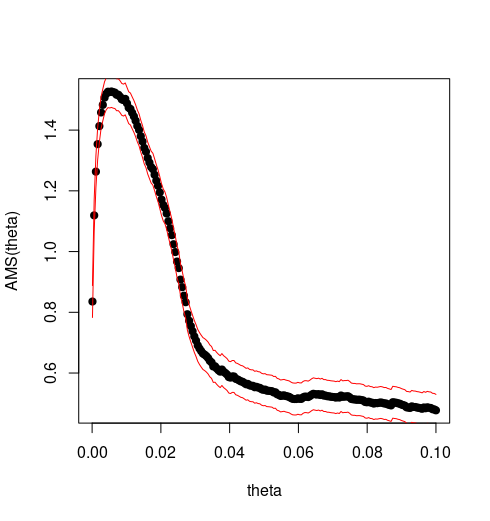
\includegraphics[scale=0.7]{../Pictures/traintunedtheta.png}
\caption{AMS values from CV procedure for different thresholds}
\label{fig: train_tuned_theta}
\end{figure}

Figure \ref{fig: train_tuned_theta} shows that AMS is maximised for small values of $\theta$ (smaller than 0.02). The maximum value of AMS is around $1.45$ - much higher than the one found with a standard logistic regression. A simple Monte carlo maximisation of $\text{AMS}(\theta)$ leads the optimal threshold $\hat{\theta}$, which is generally found to be between around $0.004$. \\

The same procedure has beed tried after PCA. Analysis of variance explained by PC's suggested to try to use a small number of PC's (see Figure \ref{fig: screeplot}).
\begin{figure}[H]
\centering
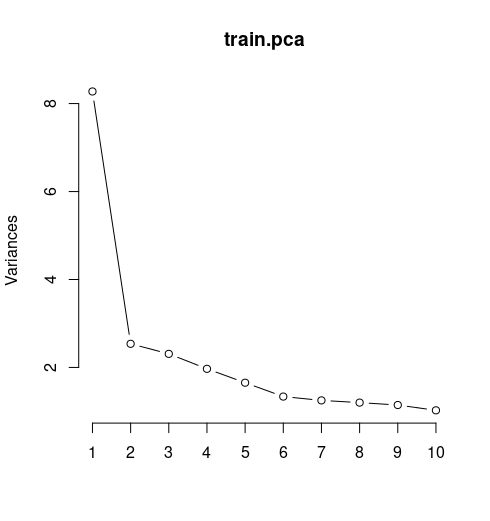
\includegraphics[scale=0.7]{../Pictures/trainpcascreeplot.png} 
\caption{Screeplot}
\label{fig: screeplot}
\end{figure}

We decided to use the first $3$ PC's as a new dataset, and repeat the procedure below. Cross-validated AMS values are plotted in Figure \ref{fig: tuned_pca}.

\begin{figure}[H]
\centering
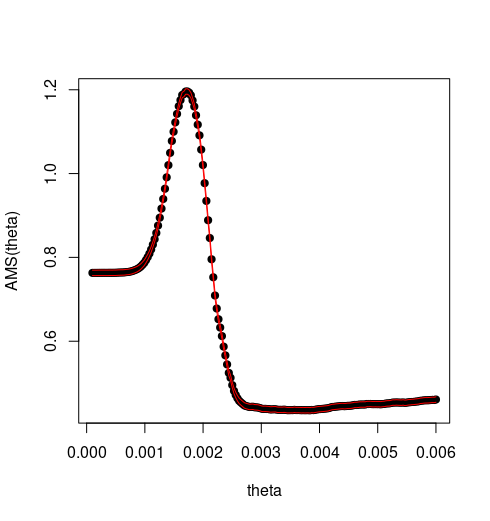
\includegraphics[scale=0.6]{../Pictures/trainpcatunedtheta.png}
\caption{AMS values from CV procedure for different thresholds - on the first three pca's}
\label{fig: tuned_pca}
\end{figure}

One can see that the AMS on validation set on the PC's is much more "peaked". In particular, AMS variance is lower than before, and the range of suitable thetas is much shorter too. This might be a sign of overfitting. $\hat{\theta}_{pc}$ is almost always $0.0017$.

\subsection{Results on test set}

It has been already said that a standard logistic regression on test set reaches an AMS of about $0.18$, which is a very low performance. \\

On the contrary, the two stage procedure has a much better performance on test set. With the threshold theta suggested from the second stage procedure on all the features, AMS on test set is about $1.5$, which is a big improvement. With the threshold suggested after PCA, we get an AMS of about $1.37$. This is still much better than using a standard logistic regression classification rule, but smaller than for the threshold suggested by the original training set. This, as said before, may be connected to some overfitting - the range of suggested theta's was much shorter than before dimensional reduction.\\

There is something else suggesting that the two-stage procedure allows us to pick a threshold which is suited for the test set too. In Figure \ref{fig: AMS on test}, AMS values from predictions on test set are plotted for different thetas. It is clear that few values of theta lead to a high value of AMS, and among them we find the ones suggested from the second stage of our procedure. 

\begin{figure}[H]
\centering
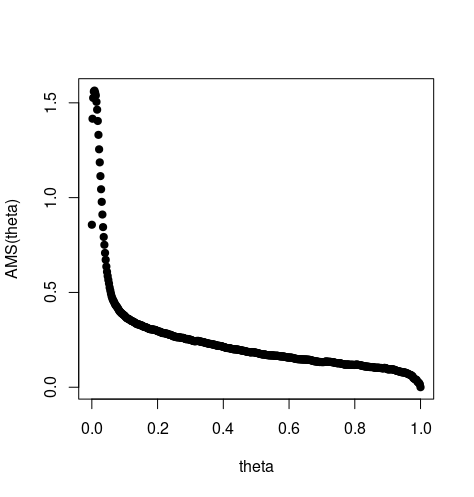
\includegraphics[scale=0.7]{../Pictures/testbadpractice.png}
\caption{AMS values after predictions on test set - for different thetas.}
\label{fig: AMS on test}
\end{figure}

\subsection{Comments}



\bibliographystyle{plain}
\bibliography{refs}

\end{document}
